 \documentclass[12pt,a4paper]{article}
\usepackage{amsmath}
\usepackage{amssymb}
\usepackage{epstopdf}
\usepackage{inputenc}
\usepackage{graphicx}
\usepackage{titletoc} 
\usepackage{fancyhdr}   
\usepackage[a4paper,pdftex]{geometry}	
\usepackage[english]{babel}
\usepackage{xcolor} 
\usepackage{enumerate}
\usepackage{fix-cm} 
\usepackage[notlof]{tocbibind}
\usepackage{amsmath}
\usepackage{listings}
\usepackage{float}
\usepackage{enumitem}
\usepackage{xcolor}
\usepackage{listings}
\usepackage{array}
\usepackage{booktabs}
\definecolor{vgreen}{RGB}{104,180,104}
\definecolor{vblue}{RGB}{49,49,255}
\definecolor{vorange}{RGB}{255,143,102}
\renewcommand\lstlistingname{Appendix}
\renewcommand\lstlistlistingname{Appendix}

\makeatletter
\newcommand*\@lbracket{[}
\newcommand*\@rbracket{]}
\newcommand*\@colon{:}
\newcommand*\colorIndex{%
	\edef\@temp{\the\lst@token}%
	\ifx\@temp\@lbracket \color{black}%
	\else\ifx\@temp\@rbracket \color{black}%
	\else\ifx\@temp\@colon \color{black}%
	\else \color{vorange}%
	\fi\fi\fi
}
\makeatother

\usepackage{trace}

\usepackage{subcaption}
\begin{document}
	\begin{titlepage}
		\begin{center}
			
\includegraphics[scale=.4]{Figures/Cover}\\
			\vspace{1cm}
			\bf{ \large {Department of Computer Science and Technology} }
		\end{center}
		
		\vspace{4cm}
		\centering
		\textbf{\Huge Deep Learning}
		\vspace{.5cm}
		
		{\Large Homework 7}

		\vspace{4cm}
		
		\textbf{\LARGE Sahand Sabour}
		
		
		
		\vspace{0.5cm}
		
		{\large 2020280401}
		
		
		\vfill
		
	\end{titlepage}
	\section*{Class Conditional Variational Autoencoder}
	In this homework, we were required to imeplement a class-conditional VAE model using the ZhuSuan library,and test it on the MNIST dataset. In the MNIST dataset, there are 10 possible labels for the samples (0-9). Binarizing the labels with the one-hot encoding method, gives a sequence of 10 digits with one 1 and nine 0s. Hence, there could be 10 locations for the 1; the probability of a label l to be one of the 10 labels L would be p(l = L) = $\frac{1}{10}$ = 0.1. According to the lecture notes, the variational lower bound for the normal case of VAE was obtained as:
	\begin{equation*}
		L(\theta, x) = E_{q(z|x)}[logp(z,x;\theta)- logq(z|x)]=E_{q(z|x)}[logp(x|z;\theta)]- KL(q(z|x)||p(z;\theta))
	\end{equation*}
	However, it can be noticed that the output of this equation is only dependent on the latent variable z and therefore, does not produce any specific results, which is not practical for our case. Hence, we should modify the lower bound to include the label l of the sample we would like to generate likewise. 
	\begin{equation*}
		L(\theta, x, l) = E_{q(z|x, l)}[logp(x, l|z;\theta)]- KL(q(z|x, l)||p(z;\theta))
	\end{equation*}
	Since $z\sim \mathcal{N}(0, 1)$ for Gaussian,  the KL-divergence is as follows:
	\begin{equation}
		- KL(q(z|x, l)||p(z;\theta)) = \frac{1}{2}(1+log\sigma^2-\mu^2-\sigma^2)
	\end{equation}
	Consequently, the expected log-likelihood would be
	\begin{equation}
		E_{q(z|x, l)}[logp(x, l|z;\theta)] = E_{q(z|x, l)}[-\sum_{j}\frac{1}{2}	log\sigma_j^2+\frac{(x_{ij}-\mu_{xi})^2}{\sigma^2}]
	\end{equation}
	Approximating the above equation with Monte Carlo methods gives
	\begin{equation}
		E_{q(z|x, l)}[logp(x, l|z;\theta)] \approx \frac{1}{L}\sum_{k}logp(x,l|z^{(k)})\quad\text{where}\quad z^{(k)} \sim q(z|x,l)
	\end{equation}
	where $z^{(k)}$ is a random variable, which cannot be used for back-propagation. Hence, by utilizing re-parameterization techniques, we have $z^{(k)} = \mu(x, l)+\sigma(x, l).\epsilon^{(k)} = g(x, l, \epsilon^{(k)})$, where g is a deep neural network. The lower bound becomes
	\begin{align*}
		L(\theta, x, l) = E_{p(\epsilon)}[log\frac{p(g(x,l,\epsilon),x;\theta)}{q(g(x,l,\epsilon)|x;\theta)}]- KL(q(z|x, l)||p(z;\theta)) \\
		L(\theta, x, l) = \frac{1}{L}\sum_{k}logp(x,l|z^{(k)}) +\frac{1}{2}\sum_{i=1}^{j}[1+log\sigma^2-\mu^2-\sigma^2]
	\end{align*}
	\begin{table}
		\centering
		\begin{tabular}{cccc}
			\toprule
			Digit & Epoch 1 & Epoch 50 & Epoch 100 \\
			\midrule
			0 & 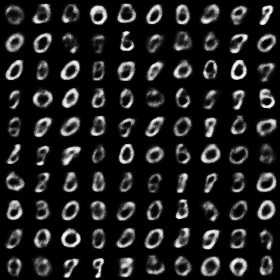
\includegraphics[width=4cm]{Figures/Epoch1_Label0} & 
\includegraphics[width=4cm]{Figures/Epoch50_Label0} & 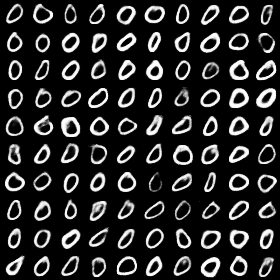
\includegraphics[width=4cm]{Figures/Epoch100_Label0}  \\
			1 & 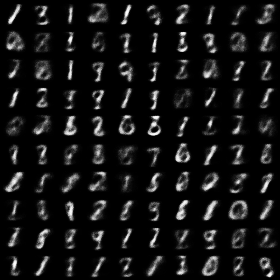
\includegraphics[width=4cm]{Figures/Epoch1_Label1} & 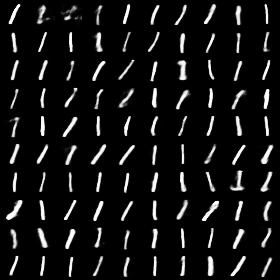
\includegraphics[width=4cm]{Figures/Epoch50_Label1} & 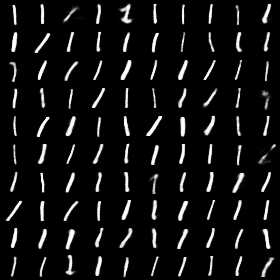
\includegraphics[width=4cm]{Figures/Epoch100_Label1}  \\
			2 & 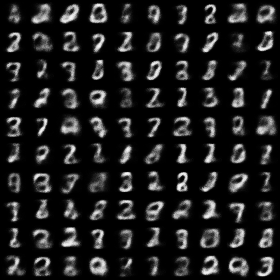
\includegraphics[width=4cm]{Figures/Epoch1_Label2} & 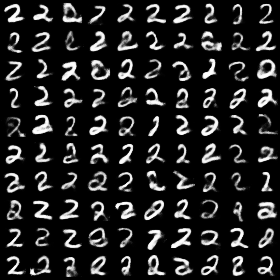
\includegraphics[width=4cm]{Figures/Epoch50_Label2} & 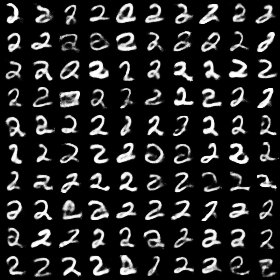
\includegraphics[width=4cm]{Figures/Epoch100_Label2}  \\
			3 & 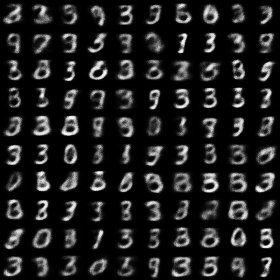
\includegraphics[width=4cm]{Figures/Epoch1_Label3} & 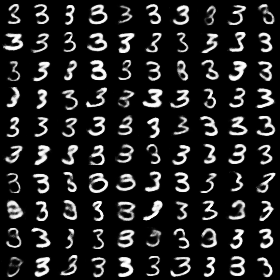
\includegraphics[width=4cm]{Figures/Epoch50_Label3} & 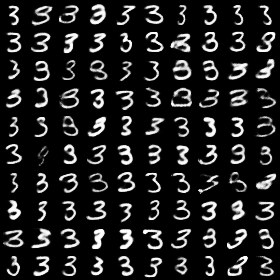
\includegraphics[width=4cm]{Figures/Epoch100_Label3}  \\
			4 & 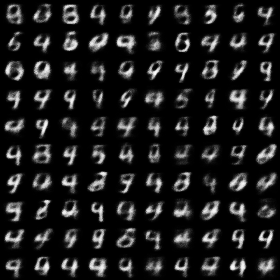
\includegraphics[width=4cm]{Figures/Epoch1_Label4} & 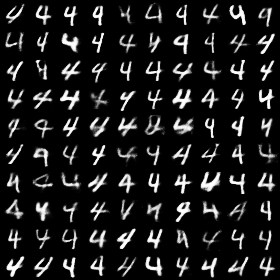
\includegraphics[width=4cm]{Figures/Epoch50_Label4} & 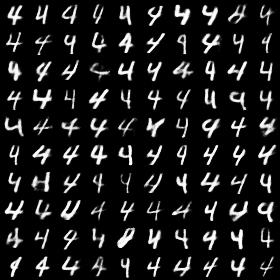
\includegraphics[width=4cm]{Figures/Epoch100_Label4}
		\end{tabular}
	\end{table}
	\begin{table}
		\centering
		\begin{tabular}{cccc}
			\toprule
			Digit & Epoch 1 & Epoch 50 & Epoch 100 \\
			\midrule
			5 & 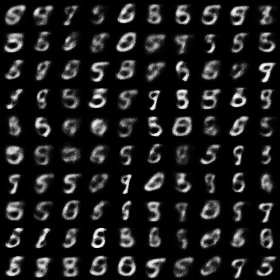
\includegraphics[width=4cm]{Figures/Epoch1_Label5} & 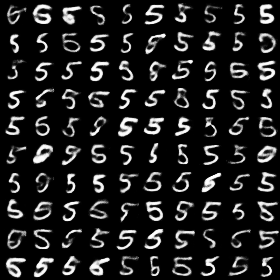
\includegraphics[width=4cm]{Figures/Epoch50_Label5} & 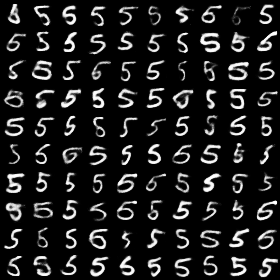
\includegraphics[width=4cm]{Figures/Epoch100_Label5}\\
			6 & 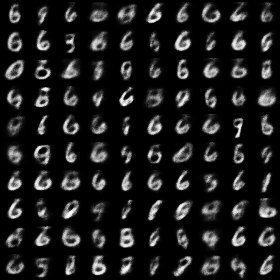
\includegraphics[width=4cm]{Figures/Epoch1_Label6} & 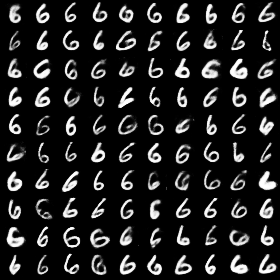
\includegraphics[width=4cm]{Figures/Epoch50_Label6} & 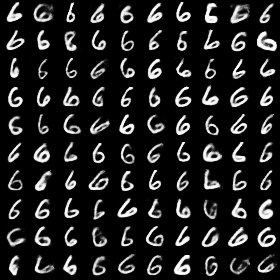
\includegraphics[width=4cm]{Figures/Epoch100_Label6}  \\
			7 & 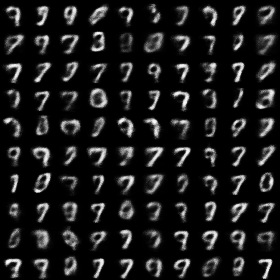
\includegraphics[width=4cm]{Figures/Epoch1_Label7} & 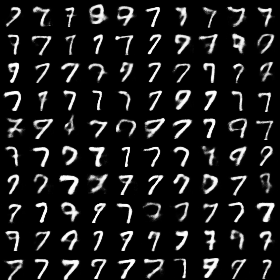
\includegraphics[width=4cm]{Figures/Epoch50_Label7} & 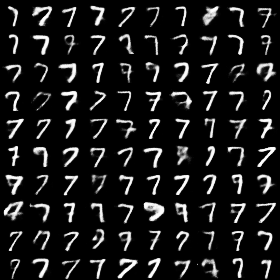
\includegraphics[width=4cm]{Figures/Epoch100_Label7}  \\
			8 & 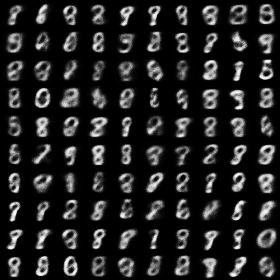
\includegraphics[width=4cm]{Figures/Epoch1_Label8} & 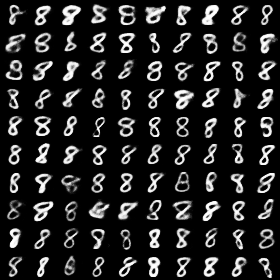
\includegraphics[width=4cm]{Figures/Epoch50_Label8} & 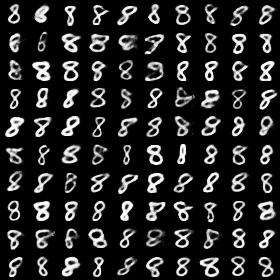
\includegraphics[width=4cm]{Figures/Epoch100_Label8}  \\
			9 & 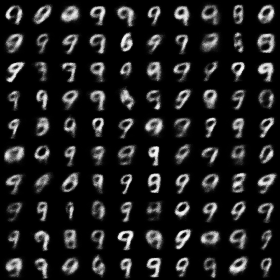
\includegraphics[width=4cm]{Figures/Epoch1_Label9} & 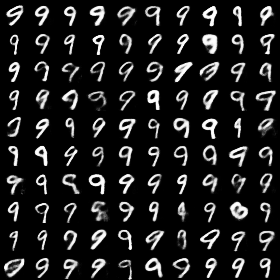
\includegraphics[width=4cm]{Figures/Epoch50_Label9} & 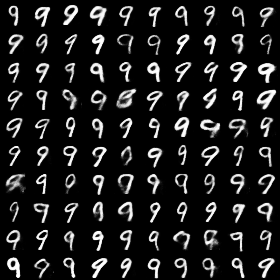
\includegraphics[width=4cm]{Figures/Epoch100_Label9}
		\end{tabular}
	\end{table}

\noindent The model was trained on the MNIST dataset and the obtained lower bound values for different number of epochs are provided respectively in the table below:
\begin{table}[H]
	\centering
	\begin{tabular}{|c|c|c|c|c|c|}
		\hline
		Epoch & 1& 10& 25& 50& 100\\\hline
		Lower Bound & -167.45& -97.954& -92.546&-90.108& -88.361\\
		\hline
	\end{tabular}
	\caption{Table of lower bound based on given epoch}
\end{table}

\noindent In addition, the obtained digit generation results are provided respectively above. Tensorflow 1.15 was used to run this implementation.
\end{document}